\subsection{Experiment 1: Initial Model Evaluation} \label{sec:exp1}

The objective of Experiment 1 was to assess the initial model's performance and to establish a baseline for future development in generative model research. The goals were to appraise the model's ability to produce realistic audio and to analyze its training process.

The initial model comprised about 4 million parameters, evenly distributed between the generator and the discriminator. The model was trained using the \ac{BCE} loss function, and no regularization techniques were applied in this experiment.

The Audio MNIST dataset was used for both training and evaluation. The Adam optimizer with a learning rate of $1 \times 10^{-4}$ was used for the generator and discriminator. Throughout the training, the generator loss was calculated as $0.487$, while the discriminator loss was measured to be $1.440$. The total loss, which is the sum of the generator and discriminator losses, was calculated to be $1.927$.

Upon evaluation, it was determined that the initial model's spectrogram did not resemble actual audio. However, the training process quickly stabilized.

Figure \ref{fig:exp1_loss} presents a line plot of the continual losses during the training process for Experiment 1, providing insight into the model's learning progress and convergence. Additionally, the spectrogram generated by the initial model is depicted in Figure \ref{fig:exp1_spectrogram}, providing a visual assessment of the audio created.

\begin{figure}[!ht]
    \centering
    \begin{subfigure}{0.45\textwidth}
        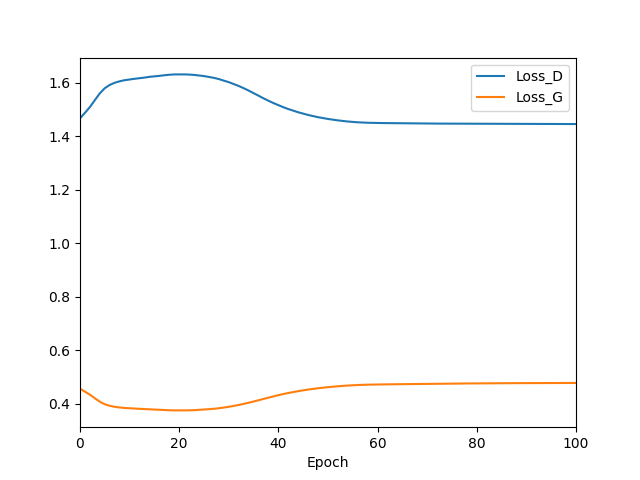
\includegraphics[width=\textwidth]{figures/4.5-results/exp1_loss.png}
        \caption{Evolving losses throughout the training process for Experiment 1.}
        \label{fig:exp1_loss}
    \end{subfigure}
    \begin{subfigure}{0.45\textwidth}
        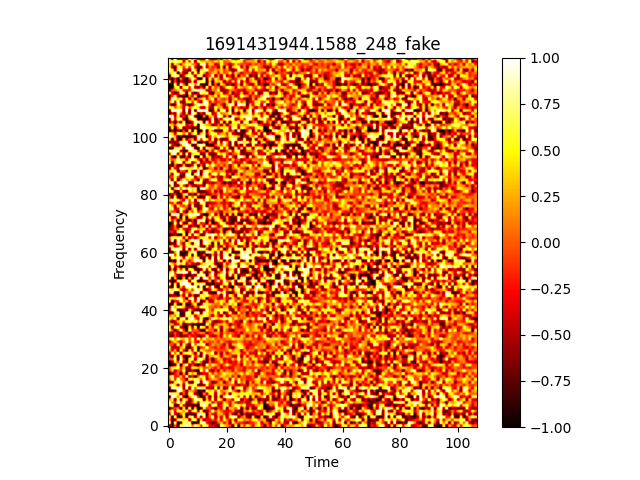
\includegraphics[width=\textwidth]{figures/4.5-results/exp1_spectrogram.png}
        \caption{Spectrogram generated in Experiment 1.}
        \label{fig:exp1_spectrogram}
    \end{subfigure}
    \caption{Results of Experiment 1.}
    \label{fig:exp1_results}
\end{figure}